\documentclass[11pt,a4paper]{article}
\usepackage[spanish,es-nodecimaldot]{babel}	% Utilizar español
\usepackage[utf8]{inputenc}					% Caracteres UTF-8
\usepackage{graphicx}						% Imagenes
\usepackage[hidelinks]{hyperref}			% Poner enlaces sin marcarlos en rojo
\usepackage{fancyhdr}						% Modificar encabezados y pies de pagina
\usepackage{float}							% Insertar figuras
\usepackage[textwidth=390pt]{geometry}		% Anchura de la pagina
\usepackage[nottoc]{tocbibind}				% Referencias (no incluir num pagina indice en Indice)
\usepackage{enumitem}						% Permitir enumerate con distintos simbolos
\usepackage[T1]{fontenc}					% Usar textsc en sections
\usepackage{amsmath}						% Símbolos matemáticos

% Comando para poner el nombre de la asignatura
\newcommand{\asignatura}{Visión por Computador}
\newcommand{\autor}{Vladislav Nikolov Vasilev}
\newcommand{\titulo}{Trabajo 1}
\newcommand{\subtitulo}{Cuestiones de teoría}
\newcommand{\answer}{\noindent\textbf{Solución}}
\newcommand{\question}[1]{\noindent\textbf{#1}}
\newcommand{\nonumbersection}[1]{\section*{#1}\addcontentsline{toc}{section}{#1}}

% Configuracion de encabezados y pies de pagina
\pagestyle{fancy}
\lhead{\autor{}}
\rhead{\asignatura{}}
\lfoot{Grado en Ingeniería Informática}
\cfoot{}
\rfoot{\thepage}
\renewcommand{\headrulewidth}{0.4pt}		% Linea cabeza de pagina
\renewcommand{\footrulewidth}{0.4pt}		% Linea pie de pagina

\begin{document}
\pagenumbering{gobble}

% Pagina de titulo
\begin{titlepage}

\begin{minipage}{\textwidth}

\centering

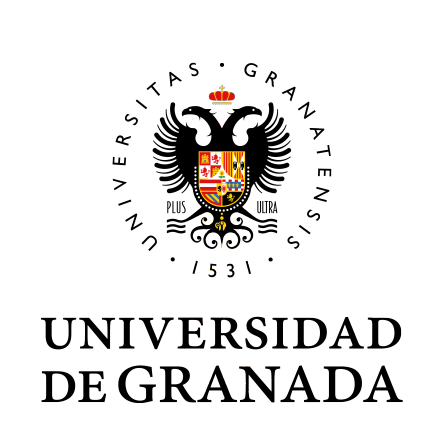
\includegraphics[scale=0.5]{img/ugr.png}\\

\textsc{\Large \asignatura{}\\[0.2cm]}
\textsc{GRADO EN INGENIERÍA INFORMÁTICA}\\[1cm]

\noindent\rule[-1ex]{\textwidth}{1pt}\\[1.5ex]
\textsc{{\Huge \titulo\\[0.5ex]}}
\textsc{{\Large \subtitulo\\}}
\noindent\rule[-1ex]{\textwidth}{2pt}\\[3.5ex]

\end{minipage}

\vspace{0.5cm}

\begin{minipage}{\textwidth}

\centering

\textbf{Autor}\\ {\autor{}}\\[2.5ex]
\textbf{Rama}\\ {Computación y Sistemas Inteligentes}\\[2.5ex]
\vspace{0.3cm}


\includegraphics[scale=0.3]{img/etsiit.jpeg}

\vspace{0.7cm}
\textsc{Escuela Técnica Superior de Ingenierías Informática y de Telecomunicación}\\
\vspace{1cm}
\textsc{Curso 2018-2019}
\end{minipage}
\end{titlepage}

\pagenumbering{arabic}
\tableofcontents
\thispagestyle{empty}				% No usar estilo en la pagina de indice

\newpage

\setlength{\parskip}{1em}

\nonumbersection{Ejercicio 1}

\question{Diga en una sola frase cuál cree que es el objetivo principal de la Visión por Computador. Diga también cuál es la
principal propiedad de las imágenes de cara a la creación de algoritmos que la procesen.}

\answer

El objetivo principal de la Visión por Computador es el procesamiento de imágenes reales o sintéticas, en movimiento
o no, mediante técnicas matemáticas y algorítmicas con el fin de poder entenderlas, valiéndose para ello de la información
semátnica y/o geométrica que puede ser extraída de dichas imágenes.

La principal propiedad de las imágenes de cara a la creación de algoritmos que la procesen es la existencia de una dependencia
entre un píxel y los píxels vecinos de éste, lo cuál implica que los vecinos de un píxel tienen un valor similar a éste. Esta
dependencia es solo local, no global; no se puede asegurar de forma cierta que exista una dependencia entre los píxels de una
región concreta y los de otra muy distante.

\nonumbersection{Ejercicio 2}

\question{Expresar las diferencias y semejanzas entre las operaciones de correlación y convolución. Dar una interpretación de
cada una de ellas que en el contexto de uso en visión por computador.}

\answer

Tanto la correlación como la convolución son operaciones que sirven para aplicar filtros lineales, los cuáles realizan
una combinación lineal de un píxel en concreto y de sus vecinos para obtener uno nuevo. Esto también implica que la salida
depende de los vecinos del píxel, y no de cómo éstos estén distribuidos. Ambas operaciones coinciden cuando la máscara
a aplicar es simétrica en ambos ejes. Además, la forma de aplicarla es la misma, ya que se va recorriendo la imágen píxel
por píxel y se aplica la operación.

Al ser ambas operaciones lineales, cumplen la propiedad de superposición, es decir, que permiten descomponer un problema
lineal complejo en uno más sencillo. Esto se puede ver de la siguiente forma:

\begin{equation}
\label{eq:superposition}
h * (f_1 + f_2) = (h * f_1) + (h * f_2)
\end{equation}

Y, además de eso, ambas operaciones son \textit{shift-invariant}, lo cuál viene a significar que la salida no depende de la
posición del vecindario, si no del vecindario como tal. Es decir, podríamos desplazar la imágen, pero el resultado sería
el mismo, solo que desplazado, en función del desplazamiento que hayamos hecho.

Sin embargo, ambas operaciones presentan algunas diferencias. La más importante de ellas es que la convolución realiza
un giro de la máscara, rotándola en cada uno de los dos ejes antes de aplicarla. Como resultado de esto, las fórmulas
de las dos operaciones son diferentes:

\begin{itemize}
	\item Para la fórmula de la correlación, la cuál se expresa como $G = H \otimes F$, siendo $F$ la imágen de entrada,
	$H$ el filtro y $G$ la imágen de salida, tenemos la siguiente expresión:
	
	\begin{equation}
		G[i, j] = \sum_{u=-k}^{k}\sum_{v=-k}^{k}H[u,v]F[i+u, j+v]
	\end{equation}
	
	\item Para la fórmula de la convolución, la cuál se expresa como $G = H \star F$, siendo $F$ la imágen de entrada,
	$H$ el filtro y $G$ la imágen de salida, tenemos la siguiente expresión:
	\begin{equation}
		G[i, j] = \sum_{u=-k}^{k}\sum_{v=-k}^{k}H[u,v]F[i-u, j-v]
	\end{equation}
\end{itemize}

Otra diferencia importante es que, al aplicar la máscara de una forma diferente, la convolución tiene algunas propiedades
extra. Algunas de ellas son, por ejemplo, la conmutatividad, la asociatividad, la identidad, entre otras.

Dentro de la visión por computador, la correlación se suele utilizar para el \textit{template matching} o búsqueda de patrones
dentro de una imágen, buscando la posición en la que se podría encontrar el patrón dentro de la imágen. La convolución,
debido a los propiedades mencionadas anteriormente, especialmente por la asociativa, es especialmente
utilizada en la aplicación de filtros que transforman la imágen, ya sean filtros de alisamiento como para detectar bordes.
Esto se debe a que permite componer filtros complejos a partir de más sencillos y aplicarlos posteriormente sobre la imágen,
en vez de ir aplicándolos uno por uno.

\nonumbersection{Ejercicio 3}

\question{¿Cuál es la diferencia ``esencial'' entre el filtro de convolución y el de mediana? Justificar la respuesta.}

\answer

La diferencia principal es que el filtro de convolución es lineal y el de mediana es no lineal. Esto significa que el filtro
de convolución utiliza una combinación lineal de los vecinos de un píxel y el píxel mismo para producir un píxel de salida.
En cambio, el filtro de mediana no hace ningún tipo de combinación lineal de los vecinos, si no que, tal y como indica su
nombre, escoge el valor mediano.

Para ver que la mediana es un filtro no lineal, vamos a probar que no cumple la propiedad de superposición (una de las propiedades
de los filtros lineales), la cuál puede ser vista en \eqref{eq:superposition}.

Para ello, vamos a suponer que tenemos dos vectores del mismo tamaño, a los cuáles llamaremos $v_1$ y $v_2$. Tenemos que
$v_1 = [3, 7, 5, 9, 4]$ y $v_2 = [2, 6, 8, 1, 3]$. Vamos a calcular cuál es la mediana de cada vector, primero por
separado y luego para la suma de los dos vectores, y veremos si coincide o no. En caso de coincidir, se cumpliría la
propiedad de superposición, y por tanto, el filtro sería lineal. En caso contrario, no se cumpliría, y no lo sería.

Tenemos que la mediana para cada vector es la siguiente:

\[mediana(v_1) = 5 \]
\[mediana(v_2) = 3 \]

Si sumamos los resultados, obtenemos:

\[mediana(v_1) + mediana(v_2) = 8\]

Ahora, vamos a ver qué resultado obtenemos para la suma de los dos vectores. Este vector tiene el siguiente valor:

\[v_1 + v_2 = [3, 7, 5, 9, 4] + [2, 6, 8, 1, 3] = [5, 13, 13, 10, 7]\]

Si obtenemos la mediana del vector resultado, obtenemos que es la siguiente:

\[mediana(v_1 + v_2) = 10\]

Y por tanto, tenemos que:

\[mediana(v_1) + mediana(v_2) \neq mediana(v_1 + v_2)\]

Por tanto, hemos probado que el filtro de mediana es no lineal, y por tanto, tiene un comportamiento diferente a la
convolución.

\nonumbersection{Ejercicio 4}

\question{Identifique el ``mecanismo concreto'' que usa un filtro de máscara para transformar una imagen.}

\answer

Los filtros utilizan la información del vecindario para transformar las imágenes. Esto es, se fijan en el píxel actual y
en sus vecinos para generar una imágen de salida con nuevos valores. Algunos de estos filtros son lineales y generan
un píxel de salida realizando una combinación lineal del píxel actual y sus vecinos. Otros, como por ejemplo el filtro
de mediana, son filtros no lineales, y devuelven el valor mediano del píxel y sus vecinos como salida.

Se utiliza este tipo de información porque, tal y como se ha dicho anteriormente, existe una dependencia entre el valor
de un píxel concreto y los valores de sus vecinos. Píxels más lejanos pueden tener otros valores, pero a efectos prácticos,
solo nos interesan aquellos que estén más cerca del píxel concreto, ya que van a tener un comportamiento similar a éste.
De esta forma, podemos saber por ejemplo cuándo hay ruido presente en la imágen, ya que nos encontraremos con píxels que tienen
valores anómalos si los comparamos con sus vecinos. Por tanto, para corregir ese ruido, podemos utilizar la información local,
promediando o aplicando el tipo de filtro más adecuado según el tipo de ruido.

\nonumbersection{Ejercicio 5}

\question{¿De qué depende que una máscara de convolución pueda ser implementada por convoluciones 1D? Justificar la respuesta.}

\answer

Para que una máscara pueda ser implementada por convoluciones 1D, ésta tiene que ser separable. Es decir, se debe de poder
descomponer como el \textit{outer-product} de dos vectores, uno fila y uno columna, los cuáles serán utilizados para
convolucionar la imágen.

Para obtenerlos, podemos utilizar la descomposición en valores singulares (\textit{SVD}). Esta descomposición viene dada
por la siguiente expresión:

\begin{equation}
\label{eq:svd}
	\mathbf{M} = \mathbf{U} \mathbf{\Sigma} \mathbf{V}^T
\end{equation}

\noindent donde $\mathbf{U}$ y $\mathbf{V}$ son matrices ortogonales y $\mathbf{\Sigma}$ es una matriz diagonal que contiene
los valores singulares de la matriz $\mathbf{M}$. Esta descomposición puede expresarse también como una suma ponderada de
matrices descomponibles de la siguiente forma:

\begin{equation}
\label{eq:svd-sum}
	\mathbf{M} = \sum_i \mathbf{A}_i = \sum_i \sigma_i \mathbf{U}_i \otimes \mathbf{V}_i
\end{equation}

\noindent donde $\sigma_i$ es el $i$-ésimo valor singular, y $\mathbf{U}_i$ y $\mathbf{V}_i$ son las $i$-ésimas columnas
de las matrices $\mathbf{U}$ y $\mathbf{V}$, respectivamente. Estas dos matrices son las mismas que se obtienen al realizar
la descomposición en valores singulares tal y como se puede ver en la ecuación \eqref{eq:svd}.

Sin embargo, a nosotros nos interesa que la matriz $\mathbf{M}$ se pueda descomponer en una única pareja de vectores
$\mathbf{U}_i$ y $\mathbf{V}_i$, para así no tener que realizar tantas operaciones. Para que esto suceda,
la matriz $\mathbf{\Sigma}$ debería tener un único valor singular, lo cuál a su vez implicaría que la matriz $\mathbf{M}$
tenga \textbf{rango 1}, ya que el rango viene dado por el número de valores singulares que se encuentren al realizar la
descomposicion. Si sucede esto, la expresión que se puede ver en \eqref{eq:svd-sum} qudaría de la siguiente forma:

\begin{equation}
	\mathbf{M} = \sigma_i \mathbf{U}_i \otimes \mathbf{V}_i
\end{equation}

\noindent siendo el índice $i$ el del único valor singular no nulo de la matriz diagonal.

De esta forma, concluimos que, para poder aplicar una máscara como convoluciones 1D, ésta tiene que ser \textbf{separable}
y de \textbf{rango 1}.

\nonumbersection{Ejercicio 6}

\question{Identificar las diferencias y consecuencias desde el punto de vista teórico y de la implementación entre:
\begin{enumerate}[label=\alph*)]
	\item Primero alisar la imagen y después calcular las derivadas sobre la
imagen alisada.
	\item Primero calcular las imágenes derivadas y después alisar dichas
imágenes.
\end{enumerate}
Justificar los argumentos.
}

\answer

Desde el punto de vista \textbf{teórico}, las dos operaciones que se describen anteriormente producen exactamente los
mismos resultados debido a la propiedad conmutativa de la convolución. Es decir, da igual el orden en el que se apliquen
los filtros ya que al final el resultado va a ser el mismo.

Desde el punto de vista de la \textbf{implementación}, aunque hemos visto que teóricamente los resultados son los mismos, el
número de operaciones que se deben hacer no son los mismos. En el primer caso se realizaría un alisamiento y $n$ cálculos
de las derivadas. Por tanto, se realizarían $n + 1$ operaciones con filtros en total. En cambio, en el segundo caso,
se realizarían primero $n$ cálculos de derivadas y, sobre cada una de las $n$ derivadas, se tendría que aplicar un filtro de
alisamiento. Por tanto, el número total de operaciones serían $2n$, lo cuál es mucho más ineficiente que el primer caso.

Por tanto, aunque desde el punto de vista teórico no exista una diferencia, hay que considerar también el punto de vista de la
implementación, ya que elegir uno u otro puede tener impactos sobre el rendimiento general del programa. Si esta operación
se tiene que aplicar para muchas imágenes, la primera opción es claramente la mejor, ya que ofrece el mismo resultado
utilizando menos convoluciones.

\nonumbersection{Ejercicio 7}

\question{Identifique las funciones de las que podemos extraer pesos correctos
para implementar de forma eficiente la primera derivada de una imagen.
Suponer alisamiento Gaussiano.}

\answer

Suponiendo que queremos calcular la derivadad de una imagen sobre la que aplicamos alisamiento Gaussiano mediante
convoluciones, esto se podría expresar de la forma $\partial(g \star f)$, donde $f$ es la imagen y $g$ el alisamiento
Gaussiano. Si aplicamos el teorema derivativo de la convolución, podemos obtener la siguiente expresión:

\begin{equation}
	\partial(g \star f) = \partial g \star f
\end{equation}

De aquí, podemos ver que es lo mismo aplicar un alisamiento Gaussiano y luego derivar el resultado que directamente aplicar
el gradiente de la Gaussiana. Por tanto, podríamos calcular la derivada de la Gaussiana y muestrearla en el rango
$[-3\sigma, 3\sigma]$, escogiendo los valores de forma acorde al tamaño de máscara. De esta forma, obtendremos los pesos
de la máscara, la cuál podríamos aplicar luego mediante convoluciones 1D, por ejemplo.

Los pèsos obtenidos serán mejores que los que pueden ofrecer ciertos operadores como Sobel o Prewitt, ya que éstos intentan
aproximar los valores de la derivada.

Al ser la Gaussiana separable, sus derivadas también lo serán. Por tanto, podemos obtener la derivada para el eje $X$ o para
el eje $Y$ de forma relativamente sencilla. Como son simétricas, lo único que cambiará es la variable que se utilice en cada
eje ($x$ o $y$, respectivamente). Por tanto, solo nos bastaría calcular la derivada de forma analítica para una de las variables.
Muestrear las derivadas posteriormente es trivial y no es costoso desde el punto de vista computacional.

\nonumbersection{Ejercicio 8}

\question{Identifique las funciones de las que podemos extraer pesos correctos
para implementar de forma eficiente la Laplaciana de una imagen. Suponer
alisamiento Gaussiano.}

\answer

Sabemos que el operador de la Laplaciana es el siguiente:

\begin{equation}
	\nabla f = \frac{\partial^2f}{\partial x^2} + \frac{\partial^2f}{\partial y^2}
\end{equation}

Si aplicamos alisamiento Gaussiano sobre la imágen, la expresión quedaría de la siguiente forma:

\begin{equation}
\label{eq:laplacian-gaussian}
	\nabla (g \star f) = \frac{\partial^2(g \star f)}{\partial x^2} + \frac{\partial^2(g \star f)}{\partial y^2}
\end{equation}

De nuevo, aplicando el teorema derivativo de la convolución, obtendríamos la siguiente expresión:

\begin{equation}
\label{eq:laplacian-efficient}
	\nabla (g \star f) = \frac{\partial^2g}{\partial x^2} \star f + \frac{\partial^2g}{\partial y^2} \star f
\end{equation}

El resultado que obtenemos en la expresión \eqref{eq:laplacian-efficient} sería el mismo que se obtendría en
la expresión \eqref{eq:laplacian-gaussian}. Por tanto, podríamos calcular las segundas derivadas parciales de la Gaussiana,
muestrear las segundas derivadas en el rango $[-3\sigma, 3\sigma]$ acorde al tamaño de la máscara. De aquí podríamos
sacar los pesos de la máscara, los cuáles pueden ser aplicados luego mediante convoluciones 1D.

Tal y como pasó antes, al ser la Gaussiana una función simétrica y separable, se puede calcular solo una de las segundas
derivadas y cambiar luego la variable utilizada. Evaluar la función resultante, de nuevo es muy sencillo, y no es muy
costoso computacionalmente. Por tanto, podríamos obtener los pesos de forma bastante eficiente.

\nonumbersection{Ejercicio 9}

\question{Suponga que le piden implementar de forma eficiente un algoritmo para
el cálculo de la derivada de primer orden sobre una imagen usando
alisamiento Gaussiano. Enumere y explique los pasos necesarios para
llevarlo a cabo.}

\answer

Para hacer una implementación de forma eficiente se podrían seguir los siguientes pasos:

\begin{enumerate}
	\item Obtener la primera derivadad de la Guassiana y muestrearla, tal y como se ha especificado en el ejercicio 7.
	\item Aplicar mediante convoluciones 1D la derivada de la Gaussina por filas y por columnas, ya que esta es separable.
	De esta forma, en vez de aplicar una convolución 2D, la cuál tiene una eficiencia de $\mathcal{O}(m^2n^2)$, teniendo una
	imagen de tamaño $m \times m$ y una máscara de tamaño $n \times n$, tendríamos dos convoluciones 1D las cuáles
	tienen una eficiencia $\mathcal{O}(m^2n)$. 
\end{enumerate}

\nonumbersection{Ejercicio 10}

\question{Identifique semejanzas y diferencias entre la pirámide gaussiana y
el espacio de escalas de una imagen, ¿cuándo usar una u otra? Justificar
los argumentos.}

\answer

Las principales semejanzas es que ambas técnicas utilizan alisamiento Gaussiano para reducir la cantidad
de ruido de la imágen, además de que ambos utilizan submuestreo para obtener imágenes más
pequeñas de la original (es decir, se escogen determinados píxels de la imágen para obtener una
más pequeña que esta) después de que se haya alisado con un filtro Gaussiano, obteniendo
por tanto distintas escalas (octavas) de la imágen.

Sin embargo, existen diferencias entre la pirámide Gaussiana y el espacio de escalas. Una de ellas es su uso.
La pirámide Gaussiana sirve para obtener distintas escalas de una imágen mediante
el alisamiento Gaussiano y el posterior submuestreo, obteniendo por tanto cada vez frecuencias más bajas de la imágen.
En cambio, el espacio de escalas se utiliza para la detección de regiones relevantes a distintas escalas. Para ello,
se vale no solo de alisar la imágen con un filtro Gaussiano, si no que también utiliza un filtro Laplaciano sobre el alisamiento
para obtener los bordes, y posteriormente, una serie de técnicas extra para determinar las regiones relevantes. Estas
operaciones se hacen en las distintas escalas para determinar regiones relevantes en cada una de ellas, ya que no serán las mismas
en imágenes más grandes que en imágenes más pequeñas. Podemos ver de alguna forma que el espacio de escalas trabaja sobre
la pirámide Gaussiana, ya que todas estas operaciones se hacen para cada escala u octava de la imágen, las cuáles pueden
ser obtenidas mediante la pirámide.


\nonumbersection{Ejercicio 11}

\question{¿Bajo qué condiciones podemos garantizar una perfecta reconstrucción
de una imagen a partir de su pirámide Laplaciana? Dar argumentos y
discutir las opciones que considere necesario.}

\answer

La imágen puede ser perfectamente reconstruida a partir de su pirámide Laplaciana, ya que todos
los pasos llevados a cabo para construirla pueden ser revertidos. Esto se debe también a que cada nivel de la pirámide
Laplaciana guarda información de las altas frecuencias que se han perdido entre un nivel de la pirámide Gaussiana y el siguiente.
En el último nivel, es decir, el más alto, se guardan las frecuencias bajas para justamente realizar la reconstrucción.

Para obtener la imágen original a partir de la pirámide, podemos partir del nivel más alto. Lo único que
tendríamos que hacer sería reescalar la imágen al tamaño del nivel anterior y aplicar un alisamiento Gaussiano para
interpolar los valores de los píxels nuevos. Ahora solo nos quedaría sumar la imagen reescalada y la del nivel anterior,
obteniendo una imágen que correspondería al nivel anterior de la pirámide Gaussiana asociada. Con esta imágen, repetimos
el proceso hasta llegar al último nivel, donde obtendremos la imágen original.

\nonumbersection{Ejercicio 12}

\question{¿Cuáles son las contribuciones más relevantes del algoritmo de
Canny al cálculo de los contornos sobre una imagen? ¿Existe alguna
conexión entre las máscaras de Sobel y el algoritmo de Canny? Justificar
la respuesta.}

\answer

El algoritmo de Canny fue una de las primeras propuestas en conseguir unos resultados muy buenos en el
cálculo de los contornos de una imagen. Antes de eso se habían producido intentos de encontrar los contornos utilizando
gradientes y eligiendo aquellos valores por encima de un umbral, pero los resultados eran, en general, bastante confusos
y malos.

El algoritmo de Canny está compuesto por una serie pasos que deben llevarse a cabo antes de conseguir el resultado
final. Estos pasos son los siguiente:

\begin{enumerate}
	\item Aplicar un filtro Gaussiano para alisar la imagen, eliminando el ruido.
	\item Calcular la orientación y la intensidad de los gradientes de la imágen. Para ello, se utiliza
	algún operador de derivada, como por ejemplo el \textbf{filtro de Sobel}, para obtener las derivadas en
	los ejes $X$ e $Y$ y posteriormente hacer los cálculos correspondientes para obtener los gradientes.
	\item Hacer la supresión de no máximos para eliminar para hacer que los bordes sean más finos, eliminando
	aquellos valores (poniéndolos a 0) que no sean máximos locales.
	\item Pasar dos umbrales: uno alto y otro bajo. Los píxels con valores inferiores al umbral bajo se eliminan. Los
	que tienen un valor superior al alto son píxels de un \textit{borde fuerte}. Si son valores intermedios, se marcan
	como píxels de \textit{borde débil}, los cuáles pueden ser causados por ruido o por dependencia de los de
	\textit{borde fuerte}.
	\item El último paso es la histéresis, donde se realiza un análisis de las regiones de los píxels de \textit{borde débil},
	mirando si están conectados a un píxel de \textit{borde fuerte}, en cuyo caso se conservan, o si no lo están, en cuyo
	caso se eliminan.
\end{enumerate}

Los tres últimos pasos fueron muy novedosos en su época, ya que no se habían probado a utilizar en la detección
de contornos. Por tanto, la técnica revolucionó la forma en la que se detectaban contornos por los buenos resultados
que permitía obtener y por su potencia y relativa sencillez.

\nonumbersection{Ejercicio 13}

\question{Identificar pros y contras de k-medias como mecanismo para crear un
vocabulario visual a partir del cual poder caracterizar patrones. ¿Qué
ganamos y que perdemos? Justificar los argumentos.}

\answer

Las ventajas de utilizar k-medias como mecanismo para crear un vocabulario visual son las siguientes:

\begin{itemize}
	\item Es un algoritmo sencillo de comprender e implementar en caso de no disponer de un \textit{framework} que lo tenga
	ya implementado.
	\item Dentro de los algoritmos de \textit{clustering}, es de los más rápidos. Tiene una complejidad en tiempo de
	$\mathcal{O}(nkdi)$, donde $n$ es el número de puntos a clasificar, $k$ el número de clústers, $d$ el número de
	dimensiones de los puntos e $i$ el número de iteraciones hasta converger.
	\item Obtiene en general unos resultados bastante buenos y que pueden ser fácilmente entendibles, ya que se agrupan
	elementos según su distancia a un determinado centroide.
	\item Puede ser ajustado a una gran variedad de problemas, convirtiéndose por tanto en una técnica flexible.
\end{itemize}

Sin embargo, no todo es perfecto. El algoritmo de k-medias también tiene sus desventajas. Algunas de ellas son las siguientes:

\begin{itemize}
	\item Los centroides iniciales se inician de forma aleatoria, con lo cuál, los resultados entre ejecuciones pueden variar.
	\item Es muy sensible a \textit{outliers}. Esto es, si dentro de un \textit{cluster} con centroide $c$ existe un punto $p$
	que está muy alejado de $c$, y el resto de elementos están muy cerca de $c$ (suponiendo que $c$ es el centroide más cercano
	a $p$), entonces este punto va a tirar mucho hacia sí el centroide del \textit{cluster} al actualizar su valor, lo cuál
	puede hacer que puntos que anteriormente estaban en el \textit{cluster} (y que deberían estarlo) dejen de pertenecer a
	este grupo de puntos. Por tanto, de alguna forma, esto puede afectar a la calidad de las soluciones encontradas.
	\item Determinar el número de \textit{clusters} a obtener puede llegar a ser complicado, ya que no hay ninguna regla escrita
	que nos permita determinar el mejor número de $k$. La clave es probar algunos valores y ver cuál es el que se ajusta
	mejor al problema concreto.
	\item Si los puntos tienen muchas dimensiones, la convergencia va a ser mucho más lenta. Esto se debe a que, al tener más
	dimensiones, los puntos tienen más opciones de distar entre sí unos de otros. Con pocas dimensiones, hay menos opciones.
\end{itemize}

Por tanto, dentro del problema de crear vocabulario visual, ganamos en rapidez y sencillez de uso y de comprensión de los
resultados. Sin embargo, nuestro mayor problema será determinar cómo de grande queremos que sea el tamaño del vocabulario (es
decir, escoger el valor de $k$), además de que deberíamos tener cuidado de que no nos encontremos demasiados \textit{outliers},
ya que estos pueden afectar a la calidad de los resultados.

\nonumbersection{Ejercicio 14}

\question{Identifique pros y contras del modelo de “Bolsa de Palabras” como
mecanismo para caracterizar el contenido de una imagen. ¿Qué ganamos y
que perdemos? Justificar los argumentos.}

\answer

\nonumbersection{Ejercicio 15}

\question{Suponga que dispone de un conjunto de imágenes de dos tipos de
clases bien diferenciadas. Suponga que conoce como implementar de forma
eficiente el cálculo de las derivadas hasta el orden N de la imagen.
Describa como crear un algoritmo que permita diferenciar, con garantías,
imágenes de ambas clases. Justificar cada uno de los pasos que proponga.}

\answer

\newpage

\begin{thebibliography}{5}

\bibitem{nombre-referencia}
Texto referencia
\\\url{https://url.referencia.com}

\end{thebibliography}

\end{document}

